\chapter{Performance}
\label{chap:Performance}

\funnyquote{There is a deep difference between what we do and what mathematicians
do. The "abstractions" we manipulate are not, in point of fact, abstract. They
are backed by real pieces of code, running on real machines, consuming real
energy and taking up real space. To attempt to completely ignore the underlying
implementation is like trying to completely ignore the laws of physics; it may
be tempting but it won't get us very far.}
{Gregor Kiczales~\cite{Kiczales92towardsa}}


\begin{figure}[htbp]
\begin{center}
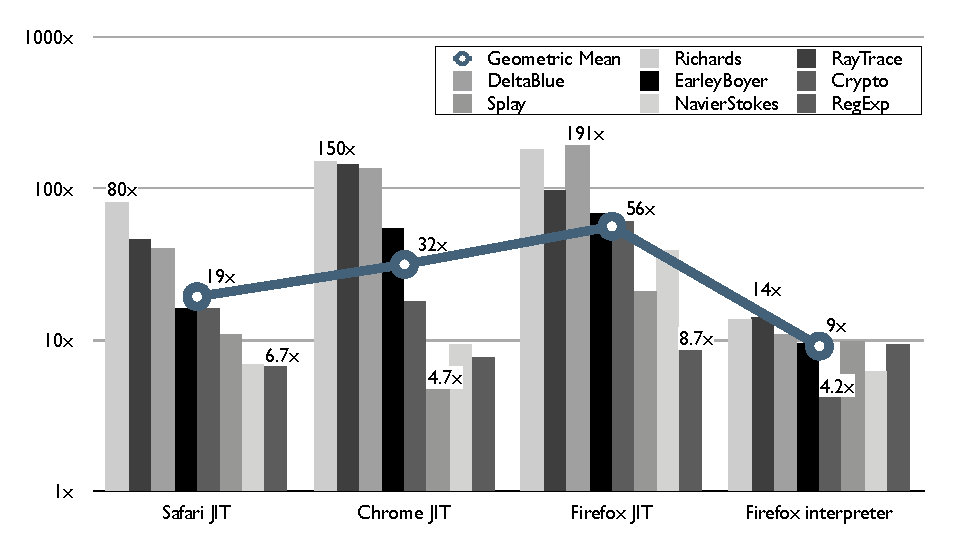
\includegraphics[width=.85\textwidth]{figures/InherentOverhead}
\caption[Inherent overhead of Photon]{Inherent overhead of Photon on the V8 benchmark suite on each JS VM.}
\label{fig:inherent-overhead-v8-benchmarks}
\end{center}
\end{figure}



\section{Setting}

\begin{itemize}

\item
{\bf Safari} version 6.0.2 (8536.26.17), which is based on the Nitro JS VM.

\item
{\bf Chrome} version 25.0.1364.172, which is based on the V8 JS VM.

\item
{\bf Firefox} version 20.0, which is based on the SpiderMonkey
JS VM.  Firefox was run with the JIT enabled, and also with
the JIT disabled (which causes the SpiderMonkey interpreter to be
used).  To disable the JIT we have used the following Firefox settings
which were suggested by the SpiderMonkey development team:

{\small
\begin{verbatim}
javascript.options.ion.content        false
javascript.options.methodjit.chrome   false 
javascript.options.methodjit.content  false
javascript.options.typeinference      false
\end{verbatim}
}

Note that disabling SpiderMonkey's type inference actually
accelerates the execution of all programs because the interpreter does
not take advantage of the type information.

\end{itemize}

To simplify the description of the results, we will conflate the name of
the web browser with that of its JS VM.

A computer with a 2.6 GHz Intel Core i7 processor and 16 GB 1600 MHz
DDR3 RAM and running OS X 10.8.2 is used in all the experiments.
Unless otherwise indicated, the values reported in the tables are the
averages over five executions.

\section{Performance with no instrumentation}


\section{Effect of send caching}

\begin{table}[t]
\centering
\begin{tabular}{|l|r|r|r|r|}
\hline
          & \multicolumn{1}{c|}{Safari} & \multicolumn{1}{c|}{Chrome} & \multicolumn{1}{c|}{Firefox} & \multicolumn{1}{c|}{Firefox} \\
Benchmark & \multicolumn{1}{c|}{JIT}    & \multicolumn{1}{c|}{JIT}    & \multicolumn{1}{c|}{JIT}     & \multicolumn{1}{c|}{interp.}     \\
\hline
Richards     &\factor{ 30.42} &\factor{ 34.15} &\factor{ 25.61} &\factor{  9.69} \\
RayTrace     &\factor{ 11.90} &\factor{ 11.11} &\factor{ 10.15} &\factor{  6.61} \\
DeltaBlue    &\factor{ 29.57} &\factor{ 33.66} &\factor{ 19.65} &\factor{ 10.55} \\
Crypto       &\factor{114.19} &\factor{171.28} &\factor{ 42.24} &\factor{ 13.57} \\
NavierStokes &\factor{195.26} &\factor{320.60} &\factor{ 98.85} &\factor{ 16.55} \\
RegExp       &\factor{  5.51} &\factor{  6.39} &\factor{  4.56} &\factor{  2.88} \\
Splay        &\factor{ 12.62} &\factor{ 28.49} &\factor{ 18.07} &\factor{  7.02} \\
\hline
{\it Geom.~mean} & \factor{\it  28.84} & \factor{\it   38.60} & \factor{\it   20.93} & \factor{\it 8.45} \\ \hline
\end{tabular}
\caption[Execution speed slowdown of Photon with deactivated send caches]{Execution speed slowdown of Photon on the V8 benchmark suite on each JS VM when send caches are deactivated}
\label{tb:send-cache-effect}
\end{table}

\section{Comparison with interpreter instrumentation}

\begin{table}[t]
\centering
\begin{tabular}{|l|r|r|r|}
\hline
          & \multicolumn{1}{c|}{Safari} & \multicolumn{1}{c|}{Chrome} & \multicolumn{1}{c|}{Firefox} \\
Benchmark & \multicolumn{1}{c|}{JIT}    & \multicolumn{1}{c|}{JIT}    & \multicolumn{1}{c|}{JIT} \\
\hline
Richards     &\factor{  1.43} &\factor{  1.84} &\factor{  2.90} \\
RayTrace     &\factor{  2.56} &\factor{  3.80} &\factor{  5.50} \\
DeltaBlue    &\factor{  1.25} &\factor{  1.50} &\factor{  3.32} \\
EarleyBoyer  &\factor{  1.03} &\factor{  1.02} &\factor{  2.80} \\
Crypto       &\factor{   .14} &\factor{   .14} &\factor{   .73} \\
Splay        &\factor{  1.36} &\factor{  1.00} &\factor{  2.26} \\
NavierStokes &\factor{   .14} &\factor{   .13} &\factor{   .50} \\
RegExp       &\factor{  1.48} &\factor{  1.54} &\factor{  3.43} \\
\hline
{\it Geom.~mean} & \factor{\it  .81} & \factor{\it  .86} & \factor{\it 2.13} \\ \hline
\end{tabular}
\caption[Performance of the V8 benchmark suite executed by Photon without instrumentation]
{Performance of the V8 benchmark suite executed by Photon without instrumentation
on each JIT VM compared to the benchmark running directly on the Firefox interpreter.  The numbers
indicate the execution speed ratio (smaller than one is better for Photon).}
\label{tb:perf-no-instrumentation-photon-vs-interpreter}
\end{table}

\section{Performance with instrumentation}

\begin{table}[t]
\centering
\begin{tabular}{|l|r|r|r|r|}
\hline
          & \multicolumn{1}{c|}{Safari} & \multicolumn{1}{c|}{Chrome} & \multicolumn{1}{c|}{Firefox} & \multicolumn{1}{c|}{Firefox} \\
Benchmark & \multicolumn{1}{c|}{JIT}    & \multicolumn{1}{c|}{JIT}    & \multicolumn{1}{c|}{JIT}     & \multicolumn{1}{c|}{interp.}     \\
\hline
Richards     &\factor{  2.31} &\factor{  2.38} &\factor{  2.81} &\factor{  1.88} \\
RayTrace     &\factor{  1.59} &\factor{  1.30} &\factor{  2.19} &\factor{  1.55} \\
DeltaBlue    &\factor{  2.68} &\factor{  3.16} &\factor{  2.03} &\factor{  1.98} \\
EarleyBoyer  &\factor{  2.18} &\factor{  2.31} &\factor{  2.71} &\factor{  1.78} \\
Crypto       &\factor{ 16.80} &\factor{ 18.53} &\factor{  6.91} &\factor{  4.33} \\
NavierStokes &\factor{ 29.17} &\factor{ 39.41} &\factor{ 11.86} &\factor{  5.65} \\
RegExp       &\factor{  1.37} &\factor{  1.31} &\factor{  1.29} &\factor{  1.30} \\
Splay        &\factor{  1.70} &\factor{  2.45} &\factor{  1.96} &\factor{  1.42} \\
\hline
{\it Geom.~mean} & \factor{\it 3.54} & \factor{\it 3.90} & \factor{\it 3.03} & \factor{\it 2.15} \\ \hline
\end{tabular}
\caption[Execution speed slowdown of Photon with a simple instrumentation]{Execution speed slowdown of Photon with the simple instrumentation of property read, write and delete}
\label{tb:slowdown-simple}
\end{table}

\begin{table}[t]
\centering
\begin{tabular}{|l|r|r|r|r|}
\hline
          & \multicolumn{1}{c|}{Safari} & \multicolumn{1}{c|}{Chrome} & \multicolumn{1}{c|}{Firefox} & \multicolumn{1}{c|}{Firefox} \\
Benchmark & \multicolumn{1}{c|}{JIT}    & \multicolumn{1}{c|}{JIT}    & \multicolumn{1}{c|}{JIT}     & \multicolumn{1}{c|}{interp.}     \\
\hline
Richards     &\factor{  1.06} &\factor{  1.26} &\factor{  1.07} &\factor{  1.24} \\
RayTrace     &\factor{  1.07} &\factor{   .93} &\factor{  1.02} &\factor{  1.15} \\
DeltaBlue    &\factor{  1.11} &\factor{  1.01} &\factor{  1.02} &\factor{  1.19} \\
EarleyBoyer  &\factor{  1.12} &\factor{  1.14} &\factor{  1.07} &\factor{  1.15} \\
Crypto       &\factor{  1.23} &\factor{  1.00} &\factor{  1.00} &\factor{  1.30} \\
NavierStokes &\factor{  1.07} &\factor{  2.05} &\factor{  1.11} &\factor{  1.36} \\
RegExp       &\factor{  1.01} &\factor{   .99} &\factor{  1.02} &\factor{  1.03} \\
Splay        &\factor{  1.68} &\factor{  1.37} &\factor{  1.05} &\factor{  1.17} \\
\hline
{\it Geom.~mean} & \factor{\it 1.15} & \factor{\it 1.18} & \factor{\it 1.04} & \factor{\it 1.19} \\ \hline
\end{tabular}
\caption[Execution speed slowdown of Photon with a fast instrumentation]{Execution speed slowdown of Photon with the fast instrumentation of property read, write and delete}
\label{tb:slowdown-fast}
\end{table}

It is common knowledge that interpreter instrumentation typically has
little impact on overall performance (see for example the
instrumentation of the JavaScriptCore VM by Richards et
al.~\cite{behavior_js}).  However, our approach is more sensitive to
instrumentation because the instrumentation code is executed by the
host JS VM.  Therefore it is important to evaluate the final
performance to ascertain Photon's general suitability for
instrumentation.

We have evaluated the performance of Photon with an instrumentation
that counts the number of run-time occurrences of the following
object representation operations: property read, write and
deletion. We chose this particular instrumentation because it is
simple, it covers frequently used object model operations and it was
actually used to gather information about JS (it can be used
to reproduce the object read, write and deletion proportion figure
from~\cite{behavior_js}).

Two implementations of this instrumentation were used; a simple and a
fast version.  The simple version does not exploit memoization and
corresponds to the straightforward implementation: incrementing a
counter and calling the corresponding object representation
operation. The fast version uses the memoization protocol to inline
the counter incrementations inside the optimized version of the object
operations.

The simple version is intended to measure the performance that can be
expected from a quickly developed instrumentation while the fast
version is intended to measure the performance impact of the
instrumentation operations alone. This is therefore a low-barrier
high-ceiling example and illustrates the flexibility that can be
gained when the choice of aiming for performance is left to users of
the system.  Not counting the result formatting code, the simple
version is 16 lines of JS code and the fast version is 100 lines of
JS code.

The execution speed slowdown of Photon with each version of the
instrumentation for each JS VM is given in
Tables~\ref{tb:slowdown-simple} and \ref{tb:slowdown-fast}.  The
average slowdown incurred by the simple version ranges from \factor{2.15} to
\factor{3.9}.  For the fast version the average slowdown ranges from \factor{1.04} to
\factor{1.19} (in other words 4\% to 19\%).  This means that on Safari JIT
and Chrome JIT, on average, the benchmarks run with the fast version
of the instrumentation on Photon essentially at the same speed as the
uninstrumented original benchmarks directly on the Firefox
interpreter.

\section{Comparison to \textit{ad hoc} program transformation}
\label{sec:esprof}

\begin{table}[t]
\centering
\begin{tabular}{|l|r|r|r|r|}
\hline
          & \multicolumn{1}{c|}{Safari} & \multicolumn{1}{c|}{Chrome} & \multicolumn{1}{c|}{Firefox} & \multicolumn{1}{c|}{Firefox} \\
Benchmark & \multicolumn{1}{c|}{JIT}    & \multicolumn{1}{c|}{JIT}    & \multicolumn{1}{c|}{JIT}     & \multicolumn{1}{c|}{interp.}     \\
\hline
Richards     &\factor{ 43.44} &\factor{ 36.74} &\factor{ 83.33} &\factor{  9.85} \\
RayTrace     &\factor{ 11.65} &\factor{ 16.46} &\factor{ 37.69} &\factor{  6.79} \\
DeltaBlue    &\factor{ 30.16} &\factor{ 42.28} &\factor{121.09} &\factor{ 10.77} \\
EarleyBoyer  &\factor{  5.67} &\factor{ 10.63} &\factor{ 23.74} &\factor{  4.82} \\
Crypto       &\factor{ 12.27} &\factor{  7.89} &\factor{ 22.32} &\factor{  3.47} \\
NavierStokes &\factor{  4.13} &\factor{  6.45} &\factor{ 15.35} &\factor{  5.17} \\
RegExp       &\factor{  2.31} &\factor{  1.65} &\factor{  3.27} &\factor{  3.33} \\
Splay        &\factor{  3.18} &\factor{  3.11} &\factor{  6.29} &\factor{  5.04} \\
\hline
{\it Geom.~mean} & \factor{\it 8.68} & \factor{\it 9.58} & \factor{\it 22.41} & \factor{\it 5.65} \\ \hline
\end{tabular}
\caption[Execution speed slowdown of esprof]{Execution speed slowdown of the V8 benchmark suite transformed by esprof
on each JIT VM}
\label{tb:esprof-slowdown}
\end{table}

As a final point of comparison, we have implemented an 
\textit{ad hoc} source-to-source transformation that reifies the same
operations as Photon, but in a more conventional way. The prototype
implementation, esprof\footnote{\url{http://github.com/dufour/esprof}}
allows instrumentations to register callbacks for various events. It does not
allow for redefining the behavior of the reified operations, but exposes that
same information to the callback as would be available in Photon. It is
important to note that esprof has not been optimized for speed. It is meant to
replicate the development effort required to implement a similar
source-to-source transformation from a set of existing code manipulation tools, and
emphasizes correctness of the transformation and ease of use over efficiency.

Table~\ref{tb:esprof-slowdown} shows the baseline performance obtained by esprof when
executing the transformed program with no instrumentation being performed.
esprof is on average between \factor{1.6} and \factor{3.3} faster than Photon.
However, this performance improvement comes at the cost of flexibility,
expressiveness and, most importantly, isolation. Because esprof only reifies
object operations performed on native JS objects, the burden of isolating the
application from the effects of the instrumentation rests solely on the
implementer of the instrumentation.

%%% \subsection{Comparison to AspectScript}
%%% 
%%% ************ MOVE (A SUMMARY OF) THESE RESULTS TO THE RELATED WORK SECTION ********************
%%% 
%%% % (safari-photon / safari-aspectscript)
%%% \begin{table}[t]
%%% \centering
%%% \begin{tabular}{|l|rr|r|}
%%% \hline
%%%           & \multicolumn{2}{c|}{V8 Score}                             &       \\
%%%           & \multicolumn{1}{c}{without} & \multicolumn{1}{c|}{with}   &       \\
%%% Benchmark & \multicolumn{1}{c}{Photon}  & \multicolumn{1}{c|}{Photon} & Ratio \\
%%% \hline
%%% DeltaBlue    &     179 &       5 &\factor{  37.21} \\
%%% NavierStokes &    2265 &       5 &\factor{ 453.73} \\
%%% RegExp       &     568 &      56 &\factor{  10.06} \\
%%% Splay        &     973 &      35 &\factor{  27.73} \\
%%% \hline
%%% {\it Geom.~mean} & {\it  688} & {\it   15} & \factor{\it 46.59} \\ \hline
%%% \end{tabular}
%%% \caption{(safari-photon / safari-aspectscript)}
%%% %\label{tb:???}
%%% \end{table}
%%% % slowdown:  GEOMEAN = 135.20  MIN = 10.06  MAX = 1233.20


